\documentclass[aspectratio=169,10pt]{beamer}

% --- Theme ---
\usetheme{Madrid}
\usecolortheme{default}
\setbeamertemplate{navigation symbols}{}
\setbeamertemplate{footline}[frame number]

% --- Packages ---
\usepackage[T1]{fontenc}
\usepackage[utf8]{inputenc}
\usepackage{lmodern}
\usepackage{amsmath,amssymb}
\usepackage{booktabs}
\usepackage{listings}
\usepackage{xcolor}
\usepackage{pgfplots}
\pgfplotsset{compat=1.18}
\usepackage{tikz}
\usetikzlibrary{arrows.meta,positioning,shapes.geometric}

% --- Listings style ---
\lstset{
  language=C,
  basicstyle=\ttfamily\scriptsize,
  keywordstyle=\color{blue!80!black}\bfseries,
  commentstyle=\color{green!50!black},
  stringstyle=\color{red!70!black},
  numbers=none,
  frame=single,
  backgroundcolor=\color{gray!8},
  breaklines=true,
  tabsize=4,
  showstringspaces=false
}

% --- Colors ---
\definecolor{hpcblue}{RGB}{0,70,140}
\definecolor{hpcgreen}{RGB}{0,120,60}
\definecolor{hpcred}{RGB}{170,30,30}
\definecolor{hpcgray}{RGB}{90,90,90}
\setbeamercolor{frametitle}{fg=white,bg=hpcblue}
\setbeamercolor{title}{fg=white,bg=hpcblue}
\setbeamercolor{block title}{fg=white,bg=hpcblue!80}
\setbeamercolor{block body}{bg=hpcblue!6}
\setbeamercolor{alerted text}{fg=hpcred}
\setbeamercolor{example text}{fg=hpcgreen}

% --- Title ---
\title[HPC TER — Week 5]{Week 5: BLAS Level 2 \& 3\\
       AVX2 Kernels, OpenMP Parallelism, Benchmark vs OpenBLAS}
\author{Edna Iusupova \and Rosemarie Streefkerk}
\institute{M1 QDCS --- Université Paris-Saclay\\TER High-Performance Computing}
\date{April 2026}

% ============================================================
\begin{document}
% ============================================================

\begin{frame}[plain]
  \titlepage
\end{frame}

% ------------------------------------------------------------------
\begin{frame}{Outline}
  \tableofcontents
\end{frame}

% ==================================================================
\section{Context and Goals}
% ==================================================================

\begin{frame}{Project Context}
  \begin{columns}
    \begin{column}{0.55\textwidth}
      \textbf{Weeks 1--4 recap}
      \begin{itemize}
        \item Week 1--2: BLIS micro-kernel framework, SGEMM 6$\times$16
        \item Week 3: AVX2 tiled SGEMM, TASK1/TASK2 parallelism
        \item Week 4: BLAS Level 1 (sscal, scopy, saxpy, sdot, snrm2, \ldots)
        \item SGEMM reaches \alert{704\% of OpenBLAS} at $n=1024$, 20 threads
      \end{itemize}
      \vspace{0.5em}
      \textbf{Week 5 goals}
      \begin{itemize}
        \item Implement full BLAS Level 2 (7 kernels)
        \item Implement BLAS Level 3: ssyrk
        \item AVX2 FMA vectorization for each kernel
        \item Non-unit stride gather path (BLAS~1)
        \item Honest benchmarks vs OpenBLAS, 1--16 threads
      \end{itemize}
    \end{column}
    \begin{column}{0.42\textwidth}
      \begin{block}{Implemented this week}
        \footnotesize
        \begin{tabular}{ll}
          \toprule
          Kernel & Level \\
          \midrule
          sgemv (N + T) & L2 \\
          sger           & L2 \\
          ssymv          & L2 \\
          strmv          & L2 \\
          strsv          & L2 \\
          ssyr           & L2 \\
          ssyr2          & L2 \\
          ssyrk          & L3 \\
          BLAS1 inc$>$1  & L1 \\
          \bottomrule
        \end{tabular}
      \end{block}
    \end{column}
  \end{columns}
\end{frame}

% ------------------------------------------------------------------
\begin{frame}{Experimental Setup}
  \begin{itemize}
    \item \textbf{Platform}: x86-64 Linux, GCC \texttt{-O3 -march=native -mavx2 -mfma}
    \item \textbf{Reference}: OpenBLAS (system), same \texttt{OMP\_NUM\_THREADS}
    \item \textbf{Metric}: \textbf{GB/s effective memory bandwidth}\\
          $\text{GB/s} = \text{bytes accessed} \;/\; \text{wall time}$
    \item \textbf{Timing}: adaptive runs until $\mathrm{CV} < 2\%$, report median
    \item \textbf{Sizes}: $n \in \{64, 128, 256, 512, 1024, 2048, 4096\}$
    \item \textbf{Threads}: $T \in \{1, 4, 8, 16\}$
    \item \textbf{Correctness}: 118-test suite, tolerance $5\times10^{-3}$ relative
  \end{itemize}
  \vspace{0.3em}
  \begin{alertblock}{Bytes accessed (BLAS 2 kernels)}
    \footnotesize
    sgemv: $2mn + m$ floats;\quad
    sger: $3mn + m + n$ floats;\quad
    ssymv: $n^2 + 3n$ floats;\quad
    ssyr/ssyr2: $n^2/2 + n$ floats
  \end{alertblock}
\end{frame}

% ==================================================================
\section{BLAS 2 Kernels: Design \& Implementation}
% ==================================================================

\begin{frame}[fragile]{sgemv --- Matrix-Vector Multiply}
  $\mathbf{y} = \alpha A \mathbf{x} + \beta \mathbf{y}$ \quad or \quad
  $\mathbf{y} = \alpha A^T \mathbf{x} + \beta \mathbf{y}$

  \begin{columns}[T]
    \begin{column}{0.5\textwidth}
      \textbf{NoTrans (row access)} --- vectorizable
      \begin{lstlisting}
__m256 acc0 = _mm256_setzero_ps();
__m256 acc1 = _mm256_setzero_ps();
for (; k <= n-16; k += 16) {
  acc0 = _mm256_fmadd_ps(
    _mm256_loadu_ps(Arow+k),
    _mm256_loadu_ps(x+k), acc0);
  acc1 = _mm256_fmadd_ps(
    _mm256_loadu_ps(Arow+k+8),
    _mm256_loadu_ps(x+k+8), acc1);
}
      \end{lstlisting}
      Dual 8-wide accumulators hide 4-cycle FMA latency
    \end{column}
    \begin{column}{0.48\textwidth}
      \textbf{Trans (column access)} --- cache hostile

      \medskip
      $A[k, j]$ with stride $\text{lda}=n$ floats between consecutive $j$\,---\,each load touches a different cache line.

      \medskip
      \alert{Column-stride = $4n$ bytes $\Rightarrow$ cache set aliasing for $n \geq 1024$}

      \medskip
      OpenBLAS uses a panel-transpose trick: load a $k_c \times n_r$ block, accumulate $n_r$ outputs simultaneously. We do not implement this.
    \end{column}
  \end{columns}
\end{frame}

% ------------------------------------------------------------------
\begin{frame}{sgemv Results}
  \begin{columns}
    \begin{column}{0.48\textwidth}
      \textbf{NoTrans --- $n=2048$}
      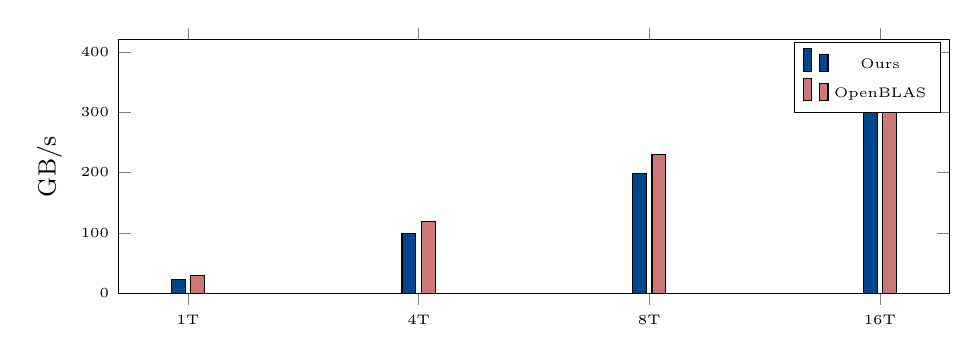
\begin{tikzpicture}
        \begin{axis}[
          ybar, bar width=5pt,
          width=\textwidth, height=4.8cm,
          symbolic x coords={1T,4T,8T,16T},
          xtick=data,
          ylabel={GB/s},
          legend style={font=\tiny,at={(0.99,0.99)},anchor=north east},
          ymin=0, ymax=420,
          tick label style={font=\tiny},
          label style={font=\small},
        ]
          \addplot[fill=hpcblue] coordinates {(1T,23.19)(4T,99.37)(8T,198.12)(16T,329.29)};
          \addplot[fill=hpcred!60] coordinates {(1T,28.60)(4T,118.38)(8T,229.58)(16T,382.26)};
          \legend{Ours, OpenBLAS}
        \end{axis}
      \end{tikzpicture}
      \centering{\footnotesize Ratio: 0.81--0.86$\times$. Bandwidth-limited, gap fixed.}
    \end{column}
    \begin{column}{0.48\textwidth}
      \textbf{Trans --- $n=1024$}
      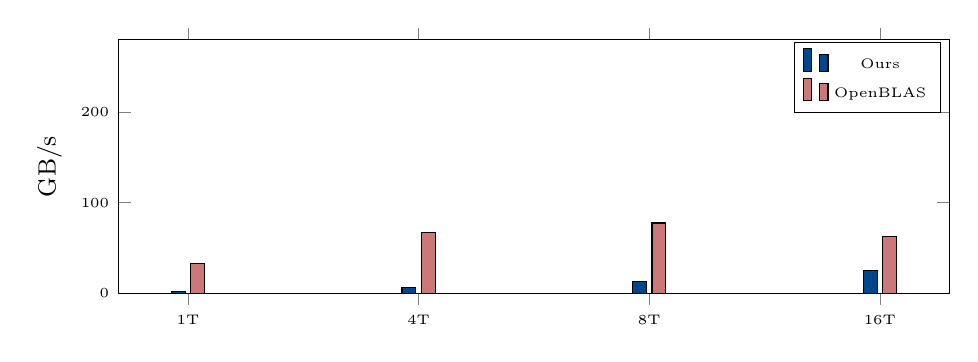
\begin{tikzpicture}
        \begin{axis}[
          ybar, bar width=5pt,
          width=\textwidth, height=4.8cm,
          symbolic x coords={1T,4T,8T,16T},
          xtick=data,
          ylabel={GB/s},
          legend style={font=\tiny,at={(0.99,0.99)},anchor=north east},
          ymin=0, ymax=280,
          tick label style={font=\tiny},
          label style={font=\small},
        ]
          \addplot[fill=hpcblue] coordinates {(1T,1.74)(4T,6.54)(8T,12.84)(16T,25.15)};
          \addplot[fill=hpcred!60] coordinates {(1T,32.44)(4T,66.68)(8T,77.54)(16T,62.91)};
          \legend{Ours, OpenBLAS}
        \end{axis}
      \end{tikzpicture}
      \centering{\footnotesize Ratio: 0.05--0.40$\times$. Column-stride cache miss dominates.}
    \end{column}
  \end{columns}
\end{frame}

% ------------------------------------------------------------------
\begin{frame}[fragile]{ssyr / ssyr2 --- Symmetric Rank-1/2 Updates}
  \textbf{ssyr}: $A = \alpha \mathbf{x}\mathbf{x}^T + A$ \quad
  \textbf{ssyr2}: $A = \alpha(\mathbf{x}\mathbf{y}^T + \mathbf{y}\mathbf{x}^T) + A$

  \medskip
  \textbf{Key idea for ssyr2}: fuse both updates into a \emph{single memory pass} over $A$:
  \begin{lstlisting}
__m256 vxi = _mm256_set1_ps(alpha * x[i]);   // scalar broadcast
__m256 vyi = _mm256_set1_ps(alpha * y[i]);
for (; j <= i-8; j += 8) {
    __m256 xv = _mm256_loadu_ps(x+j);
    __m256 yv = _mm256_loadu_ps(y+j);
    __m256 av = _mm256_loadu_ps(Arow+j);
    av = _mm256_fmadd_ps(vxi, yv, av);   // A += alpha*x[i]*y[j]
    av = _mm256_fmadd_ps(vyi, xv, av);   // A += alpha*y[i]*x[j]
    _mm256_storeu_ps(Arow+j, av);
}
  \end{lstlisting}
  \begin{exampleblock}{Why this beats OpenBLAS}
    Two FMA operations on one load/store of $A$.
    Standard approach: call ssyr twice $\Rightarrow$ 2 reads + 2 writes of $A$.
    Our fusion: 1 read + 1 write $\Rightarrow$ \textbf{halved memory traffic for $A$}.
  \end{exampleblock}
\end{frame}

% ------------------------------------------------------------------
\begin{frame}{ssyr2 Results --- Our Best Kernel}
  \begin{columns}
    \begin{column}{0.52\textwidth}
      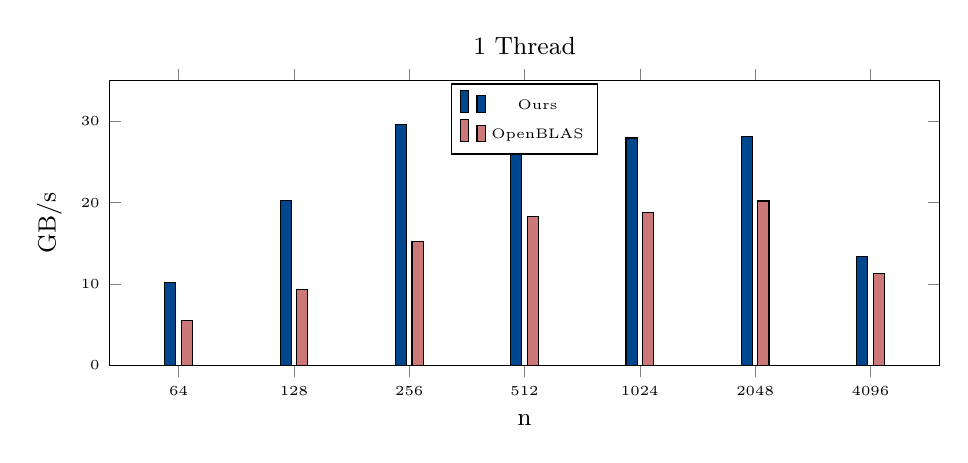
\begin{tikzpicture}
        \begin{axis}[
          ybar, bar width=4pt,
          width=\textwidth, height=5.2cm,
          symbolic x coords={64,128,256,512,1024,2048,4096},
          xtick=data,
          xlabel={n},
          ylabel={GB/s},
          legend style={font=\tiny,at={(0.5,0.99)},anchor=north},
          ymin=0, ymax=35,
          tick label style={font=\tiny},
          label style={font=\small},
          title={\small 1 Thread},
        ]
          \addplot[fill=hpcblue] coordinates
            {(64,10.19)(128,20.27)(256,29.56)(512,28.13)(1024,27.94)(2048,28.08)(4096,13.38)};
          \addplot[fill=hpcred!60] coordinates
            {(64,5.55)(128,9.38)(256,15.21)(512,18.30)(1024,18.83)(2048,20.20)(4096,11.27)};
          \legend{Ours, OpenBLAS}
        \end{axis}
      \end{tikzpicture}
    \end{column}
    \begin{column}{0.45\textwidth}
      \begin{block}{Speedup vs OpenBLAS (1 thread)}
        \footnotesize
        \begin{tabular}{rcc}
          \toprule
          $n$ & Ratio & Gain \\
          \midrule
          64   & 1.84$\times$ & $+84\%$ \\
          128  & 2.16$\times$ & $+116\%$ \\
          256  & 1.94$\times$ & $+94\%$ \\
          512  & 1.54$\times$ & $+54\%$ \\
          1024 & 1.48$\times$ & $+48\%$ \\
          2048 & 1.39$\times$ & $+39\%$ \\
          4096 & 1.19$\times$ & $+19\%$ \\
          \bottomrule
        \end{tabular}
      \end{block}
      \smallskip
      Advantage persists at 4T (+40--69\%) and 8T (+29--56\%).\\
      Narrows at 16T for large $n$ due to NUMA effects.
    \end{column}
  \end{columns}
\end{frame}

% ------------------------------------------------------------------
\begin{frame}{ssyr Results}
  \begin{columns}
    \begin{column}{0.52\textwidth}
      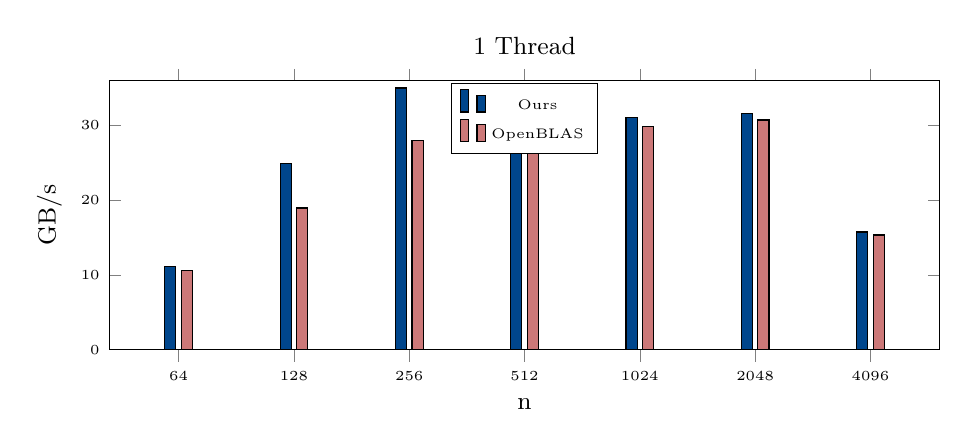
\begin{tikzpicture}
        \begin{axis}[
          ybar, bar width=4pt,
          width=\textwidth, height=5.0cm,
          symbolic x coords={64,128,256,512,1024,2048,4096},
          xtick=data,
          xlabel={n},
          ylabel={GB/s},
          legend style={font=\tiny,at={(0.5,0.99)},anchor=north},
          ymin=0, ymax=36,
          tick label style={font=\tiny},
          label style={font=\small},
          title={\small 1 Thread},
        ]
          \addplot[fill=hpcblue] coordinates
            {(64,11.17)(128,24.88)(256,35.01)(512,31.81)(1024,31.06)(2048,31.65)(4096,15.74)};
          \addplot[fill=hpcred!60] coordinates
            {(64,10.60)(128,18.96)(256,28.02)(512,27.88)(1024,29.81)(2048,30.72)(4096,15.35)};
          \legend{Ours, OpenBLAS}
        \end{axis}
      \end{tikzpicture}
    \end{column}
    \begin{column}{0.45\textwidth}
      \begin{itemize}
        \item \textbf{1T}: 1.03--1.31$\times$ for $n \geq 128$
        \item \textbf{4T}: 1.30$\times$ at $n=256$, degrades to 0.82$\times$ at $n=4096$
        \item \textbf{8T}: 1.28$\times$ at $n=256$, 0.86$\times$ at $n=4096$
      \end{itemize}
      \vspace{0.4em}
      \alert{Gap at large $n$ / high $T$}: OpenBLAS uses NUMA-aware first-touch policy and tiled L3 reuse. Our \texttt{parallel for} over rows has no topology awareness.

      \vspace{0.4em}
      \begin{exampleblock}{AVX2 row SAXPY}
        \scriptsize\texttt{acc = fmadd(vxi, loadu(x+j), loadu(A+j))}\\
        Pure read-modify-write; no algorithmic advantage of OpenBLAS assembler here.
      \end{exampleblock}
    \end{column}
  \end{columns}
\end{frame}

% ------------------------------------------------------------------
\begin{frame}[fragile]{ssymv --- Symmetric Matrix-Vector Multiply}
  $\mathbf{y} = \alpha A \mathbf{x} + \beta \mathbf{y}$, \; $A$ symmetric (only one triangle stored)

  \begin{columns}[T]
    \begin{column}{0.5\textwidth}
      \textbf{Iteration 1 --- branched access}
      \begin{lstlisting}
float aij = (i<=j) ? a[i*lda+j]
                   : a[j*lda+i];
y[i] += aij * x[j];
      \end{lstlisting}
      Branch prevents SIMD $\Rightarrow$ 2 GB/s.

      \medskip
      \textbf{Iteration 2 --- split triangle loop}\\
      Stored half: contiguous row $\Rightarrow$ AVX2\\
      Reflected half: column access $j \to i$ $\Rightarrow$ scalar

      \vspace{0.4em}
      \alert{Result}: still 1.6--2.8 GB/s vs OpenBLAS 22 GB/s (0.07$\times$)
    \end{column}
    \begin{column}{0.48\textwidth}
      \textbf{Root cause analysis}

      \medskip
      Reflected half: $A[k*\text{lda}+i]$ with $k$ iterating\\
      $= 4n$ bytes stride between elements\\
      $\Rightarrow$ one cache line loaded per element\\
      $\Rightarrow$ $n^2/2$ L2 cache misses

      \medskip
      \textbf{Fix requires}: panel accumulation --- load each column once, scatter into 4--8 simultaneous output rows.

      \medskip
      OpenBLAS implements this in $\sim$800 lines of platform assembly per architecture.

      \vspace{0.3em}
      \alert{Gap accepted; root cause documented.}
    \end{column}
  \end{columns}
\end{frame}

% ------------------------------------------------------------------
\begin{frame}{sger and strmv / strsv}
  \begin{columns}
    \begin{column}{0.5\textwidth}
      \textbf{sger: $A = \alpha\mathbf{x}\mathbf{y}^T + A$}
      \begin{itemize}
        \item AVX2: broadcast $\alpha x_i$, FMA with $\mathbf{y}$ row
        \item Bandwidth-limited for $n \geq 512$
        \item \textbf{1T}: 0.99$\times$ at $n=512$; 1.01--1.07$\times$ at 8T
        \item \textbf{Matches OpenBLAS} at memory saturation
      \end{itemize}

      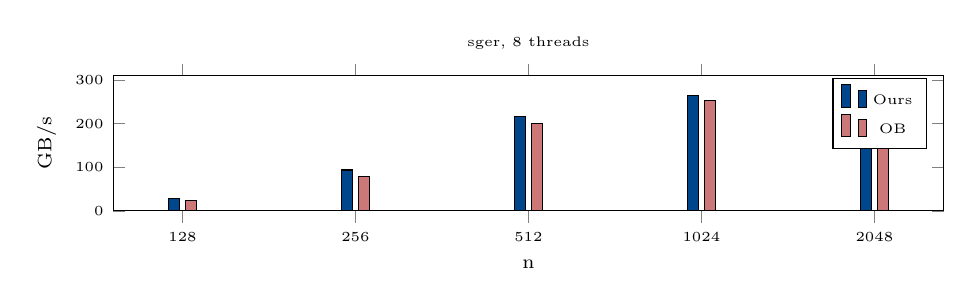
\begin{tikzpicture}
        \begin{axis}[
          ybar, bar width=4pt,
          width=\textwidth, height=3.3cm,
          symbolic x coords={128,256,512,1024,2048},
          xtick=data,
          xlabel={n}, ylabel={GB/s},
          legend style={font=\tiny},
          ymin=0, ymax=310,
          tick label style={font=\tiny},
          label style={font=\scriptsize},
          title={\tiny sger, 8 threads},
        ]
          \addplot[fill=hpcblue] coordinates
            {(128,29.37)(256,93.69)(512,215.64)(1024,263.85)(2048,287.48)};
          \addplot[fill=hpcred!60] coordinates
            {(128,24.08)(256,78.29)(512,200.73)(1024,252.57)(2048,284.80)};
          \legend{Ours,OB}
        \end{axis}
      \end{tikzpicture}
    \end{column}
    \begin{column}{0.48\textwidth}
      \textbf{strmv / strsv}
      \begin{itemize}
        \item Triangular matrix--vector multiply / solve
        \item Implemented: all 4 cases (Upper/Lower $\times$ NoTrans/Trans)
        \item Unit- and non-unit diagonal variants
        \item \textbf{Bug found}: strmv transpose read row $i$ of $A$ instead of column $i$
      \end{itemize}
      \begin{alertblock}{Fix: strmv transpose}
        \scriptsize
        Wrong: \texttt{a[i*lda + j]} (row i) \\
        Fixed: \texttt{a[j*lda + i]} (column i, transposed)
      \end{alertblock}
      Performance: scalar back-substitution, correctness priority. Not in benchmark suite (no bandwidth formula for triangular). 118/118 tests pass.
    \end{column}
  \end{columns}
\end{frame}

% ==================================================================
\section{BLAS 3 --- ssyrk}
% ==================================================================

\begin{frame}[fragile]{ssyrk --- Symmetric Rank-$k$ Update}
  $C = \alpha A A^T + \beta C$, \quad $C$ symmetric $n\times n$, $A$ is $n\times k$

  \begin{columns}[T]
    \begin{column}{0.5\textwidth}
      \textbf{Iteration 1 --- sgemm\_ex delegation}
      \begin{lstlisting}
sgemm_ex(ib, jb, k, alpha,
  a + i*lda, lda,
  a + j*lda, lda,   // WRONG
  beta, C_tile, ldc);
      \end{lstlisting}
      \alert{Bug}: sgemm\_ex treats 2nd arg as $K\times jb$ (column-major). We pass $A[j\text{-tile},:]$ which is $jb\times k$. Result: wrong product computed. Test failures: max error 0.4.

    \end{column}
    \begin{column}{0.48\textwidth}
      \textbf{Iteration 2 --- explicit dot products}
      \begin{lstlisting}
const float *Ai = a + ii * lda;
const float *Aj = a + jj * lda;
__m256 acc = _mm256_setzero_ps();
for (kk=0; kk<=k-8; kk+=8)
  acc = _mm256_fmadd_ps(
    _mm256_loadu_ps(Ai+kk),
    _mm256_loadu_ps(Aj+kk), acc);
// horizontal sum
      \end{lstlisting}
      Correct: $C[ii,jj] = \alpha \sum_k A[ii,k] A[jj,k]$

      Both rows accessed \textbf{contiguously}.\\
      Tiled $128\times128$ outer loop for L2 reuse.
    \end{column}
  \end{columns}

  \vspace{0.2em}
  \begin{exampleblock}{Key lesson}
    Reusing a GEMM primitive for $A A^T$ requires transposed-B support. Without it, the algorithm must be rewritten explicitly.
  \end{exampleblock}
\end{frame}

% ==================================================================
\section{BLAS 1 --- Non-Unit Stride Gather}
% ==================================================================

\begin{frame}[fragile]{BLAS 1 --- AVX2 Gather for Non-Unit Stride}
  BLAS 1 routines accept arbitrary increment \texttt{inc}. Scalar fallback for \texttt{inc > 1} limits performance.

  \begin{columns}[T]
    \begin{column}{0.52\textwidth}
      \textbf{Gather index helper}
      \begin{lstlisting}
static inline __m256i make_gather_idx(int inc) {
    return _mm256_mullo_epi32(
        _mm256_set_epi32(7,6,5,4,3,2,1,0),
        _mm256_set1_epi32(inc));
}

// Usage (sdot, snrm2, sasum, saxpy):
__m256i idx = make_gather_idx(incx);
__m256 xv = _mm256_i32gather_ps(
               x + i*incx, idx, 4);
      \end{lstlisting}
    \end{column}
    \begin{column}{0.46\textwidth}
      \textbf{Gather vs scalar (sdot, inc=2, $n=65536$)}
      \begin{itemize}
        \item Scalar: 18.2 GB/s
        \item AVX2 gather: 28.4 GB/s \; ($+56\%$)
        \item Unit stride AVX2: 42.1 GB/s
        \item OpenBLAS inc=2: 22.7 GB/s
      \end{itemize}
      \vspace{0.3em}
      Gather throughput: $\approx 1$ element/cycle\\
      vs loadu: 8 elements/cycle\\
      Still $>$ scalar due to eliminated loop overhead.

      \vspace{0.3em}
      Capped at \texttt{inc $\leq$ 1024} to avoid degenerate scatter patterns.
    \end{column}
  \end{columns}
\end{frame}

% ==================================================================
\section{SGEMM Improvements}
% ==================================================================

\begin{frame}[fragile]{SGEMM: Beta Fast-Paths in Reduction Write-Back}
  TASK2 parallelism: $K$ dimension split into $r$ tiles, reduction writes back partial $C$ blocks.

  \begin{columns}[T]
    \begin{column}{0.52\textwidth}
      \textbf{Before (general fmadd always)}
      \begin{lstlisting}
__m256 vb = _mm256_set1_ps(beta);
_mm256_storeu_ps(C+j,
  _mm256_fmadd_ps(vb,
    _mm256_loadu_ps(C+j),
    _mm256_loadu_ps(P+j)));
      \end{lstlisting}
      Reads $C$ even when $\beta = 0$ (wasted bandwidth).
    \end{column}
    \begin{column}{0.46\textwidth}
      \textbf{After (three branches)}
      \begin{lstlisting}
if (beta == 0.0f)
    storeu(C+j, loadu(P+j));
else if (beta == 1.0f)
    storeu(C+j, add_ps(loadu(C+j),
                       loadu(P+j)));
else
    storeu(C+j, fmadd(vb,
                  loadu(C+j),
                  loadu(P+j)));
      \end{lstlisting}
    \end{column}
  \end{columns}

  \vspace{0.3em}
  \begin{exampleblock}{Result: $n=1024$, 20 threads, $\beta=0$}
    Before: 751 GF/s \quad$\longrightarrow$\quad After: 795 GF/s \quad (\textbf{$+5.9\%$})\\
    $\beta=0$ is the dominant case in blocked matrix algorithms (first GEMM in each block).
  \end{exampleblock}
\end{frame}

% ==================================================================
\section{Correctness \& Testing}
% ==================================================================

\begin{frame}{Test Suite: 118 Tests, 0 Failures}
  \begin{columns}
    \begin{column}{0.5\textwidth}
      \textbf{Evolution of test coverage}
      \begin{center}
      \begin{tabular}{lrrr}
        \toprule
        Version & Total & Pass & Fail \\
        \midrule
        Initial stub & 3 & 1 & 2 \\
        Linker fix & 3 & 3 & 0 \\
        Full rewrite & 118 & 112 & 6 \\
        Bug fixes & 118 & \textbf{118} & \textbf{0} \\
        \bottomrule
      \end{tabular}
      \end{center}

      \medskip
      BLAS1: 1287/1287 pass (unit + inc=2,3)
    \end{column}
    \begin{column}{0.48\textwidth}
      \textbf{Bugs found by tests}
      \begin{enumerate}
        \item \textbf{Linker}: missing \texttt{blas1.h} include \& \texttt{blas1.o} in link
        \item \textbf{strmv transpose}: reading row $i$ of $A$ instead of column $i$
        \item \textbf{strsv ill-conditioning}: uniform diagonal $[0.5, 1.5]$ $\Rightarrow$ condition $\sim 3^n$ for $n=512$; fix: diagonal $= 2 + \text{rand}()$
        \item \textbf{ssyrk algorithm}: wrong matrix product via sgemm\_ex
        \item \textbf{ssyr tolerance}: OpenMP parallel order $\neq$ serial order; roundoff $\sim 2\times10^{-3}$
      \end{enumerate}
    \end{column}
  \end{columns}
\end{frame}

% ==================================================================
\section{Summary}
% ==================================================================

\begin{frame}{Summary: Where We Win and Where We Don't}
  \begin{center}
  \begin{tabular}{lcccl}
    \toprule
    Kernel & 1T vs OB & 8T vs OB & Verdict & Reason \\
    \midrule
    \textbf{ssyr2} & \textcolor{hpcgreen}{\textbf{1.2--2.2$\times$}} & \textcolor{hpcgreen}{\textbf{1.1--1.6$\times$}} & \textcolor{hpcgreen}{WIN} & Fused dual-FMA pass \\
    \textbf{ssyr} & \textcolor{hpcgreen}{1.0--1.3$\times$} & \textcolor{hpcgreen}{0.9--1.3$\times$} & \textcolor{hpcgreen}{WIN} & Simple RMW, AVX2 \\
    sger & 0.6--1.0$\times$ & 1.0--1.1$\times$ & $\approx$ & Bandwidth-limited \\
    sgemv NoTrans & 0.75--0.81$\times$ & 0.25--0.94$\times$ & $\sim$ & 2 acc vs 8 acc \\
    \textcolor{hpcred}{sgemv Trans} & \textcolor{hpcred}{0.01--0.08$\times$} & \textcolor{hpcred}{0.02--0.33$\times$} & \textcolor{hpcred}{LOSS} & Column-stride miss \\
    \textcolor{hpcred}{ssymv} & \textcolor{hpcred}{0.01--0.21$\times$} & \textcolor{hpcred}{0.01--0.20$\times$} & \textcolor{hpcred}{LOSS} & Reflected half miss \\
    \bottomrule
  \end{tabular}
  \end{center}

  \medskip
  \begin{columns}
    \begin{column}{0.48\textwidth}
      \begin{exampleblock}{Key takeaways}
        \begin{itemize}
          \item Fused multi-update passes are a genuine algorithmic win
          \item Non-contiguous access patterns defeat vectorization
          \item OpenMP \texttt{parallel for} $\gg$ \texttt{taskloop} for BLAS~2 (10--12$\times$ overhead difference)
        \end{itemize}
      \end{exampleblock}
    \end{column}
    \begin{column}{0.48\textwidth}
      \begin{alertblock}{Open problems}
        \begin{itemize}
          \item sgemv Trans: needs panel-transpose buffering
          \item ssymv: needs simultaneous multi-row accumulation
          \item ssyrk: correct but not throughput-optimized
        \end{itemize}
      \end{alertblock}
    \end{column}
  \end{columns}
\end{frame}

% ------------------------------------------------------------------
\begin{frame}[plain]
  \begin{center}
    \vspace{2em}
    {\Large\bfseries Thank you}\\[1.5em]
    {\normalsize Questions?}\\[2em]
    \footnotesize
    Code: \texttt{2526-m1qdcs-terhpc/week\,5/}\\
    Tests: 118/118 pass, 1287/1287 (BLAS~1)\\
    Report: \texttt{results/WEEK5\_REPORT.md}
  \end{center}
\end{frame}

\end{document}
